\newpage
\subsection{Optimization results}  
In this section, we present the results of the optimization studies on the Model 1 configuration using the Nelder--Mead and MADS methods. The objective functions considered are the near-wall shear rate and the turbulent kinetic energy. Our primary goals are to validate the optimization framework, evaluate the convergence of both optimization methods used, and compare their efficiency. Detailed specifications of the hardware used for these computations can be found in \cite{gpu}.

The custom Nelder--Mead implementation was parallelized and executed on four dedicated compute nodes, managed through a Slurm-based job submission system \cite{slurm}. This setup enabled multiple function evaluations to be performed simultaneously, naturally reducing the total wall time for the optimization process. In contrast, the MADS method was not parallelized and ran sequentially on a single computational node.

To ensure that the optimized configurations remained physiologically meaningful, we imposed constraints on the offset parameter \(o_1\). First, a primary constraint defined the feasible offset range as \(0{,}0 \leq o_1 \leq 2{,}4\,\text{cm}\). Next, to achieve the clinically motivated target (discussed in Section~\ref{objective funcs meaning}) that at least 25\% of the IVC blood flow must be directed into the LPA, we refined the constraint further. Using precomputed splits to identify offsets that satisfied this flow distribution, the offset was ultimately constrained to \(0{,}0 \leq o_1 \leq 0{,}78\,\text{cm}\), as shown in Figure~\ref{fig:ivc_flow_split}.

The sampled data points in Figure~\ref{fig:summary_metrics} did not cover the entirety of the feasible set and were interpolated linearly, hence determining the exact minima of the objective functions is not possible. However, the data strongly suggests that under the given constraints, the minimum near-wall shear rate is located near the upper bound of the feasible set, i.e. near \(o_1 = 0{,}78\,\text{cm}\). The minimum turbulent kinetic energy appears to be located near the lower bound, i.e. near \(o_1 = 0{,}0\,\text{cm}\). Finally, the initial starting point for the optimization was chosen at the center of the feasible set, \(o_1^\text{init} = 0{,}39\,\text{cm}\). 

In the following studies, we focus on both the number of function evaluations ($\#f$) and the total wall time required. Here, $\#f$ corresponds to the number of simulation runs needed. Because the custom Nelder–Mead implementation supports parallel execution of these simulations, it can complete a larger number of evaluations in a shorter wall time compared to MADS, which operates sequentially. The longer runtime associated with the MADS approach makes it more computationally demanding. To avoid excessive runtimes, MADS was run with a preset cap of 20 on $\#f$, ensuring that the total computation time remained manageable.

\begin{table}[H]
	\bgroup
	\centering
	\setlength\tabcolsep{3mm}
	\def\arraystretch{2.2}%
	\begin{tabular}{|c|c|c|}
		\hline
		\textbf{Method} & \textbf{Objective function} & \textbf{Page} \\ \hline
		Nelder-Mead & $\dot{\gamma}^{A}_{\mathrm{nw}}$ &\hyperlink{page.60}{60} \\ \hline
		Nelder-Mead & $T^{A}_{\mathrm{turb}}$ & \hyperlink{page.61}{61} \\ \hline
		MADS & $\dot{\gamma}^{A}_{\mathrm{nw}}$ & \hyperlink{page.62}{62} \\ \hline
		MADS & $T^{A}_{\mathrm{turb}}$ & \hyperlink{page.63}{63} \\ \hline
	\end{tabular}
	\caption{List of studied optimization configurations.}
	\label{tab:optim configs}
	\egroup
\end{table}

\newpage
\begin{optimproblem}{Basic cylindrical junction ($\dot{\gamma}^{A}_{\text{nw}}$)}
	\vspace{2mm}
	Objective:  Minimizing near-wall shear rate $\dot{\gamma}^{A}_{\text{nw}}$.
	
	\vspace{2mm}
	Geometrical model:
	\begin{itemize}
		\item Model 1 as described in Section~\ref{mod:model1}.
		\item Optimization parameters: offset $o_1$.
	\end{itemize}
	Constraints:
	\begin{itemize}
		\item Offset constraint: $0{,}0~\text{cm} \leq o_1 \leq 2{,}4~\text{cm}$.
		\item Flow split constraint: $F^{\text{LPA}}_{\text{IVC}} \geq 25~\%$.
	\end{itemize}
	Optimization method:
	\begin{itemize}
		\item Nelder-Mead method as described in Section~\ref{framework} and Appendix~\ref{appendix C}.
	\end{itemize}
	Initial point: $o^{\text{init}}_{1}$ = 0{,}39 cm
	\label{optimprob:1}
\end{optimproblem}
\vspace{-5mm}

\begin{figure}[H]
	\centering
	\begin{subfigure}{0.46\textwidth}
		\centering
		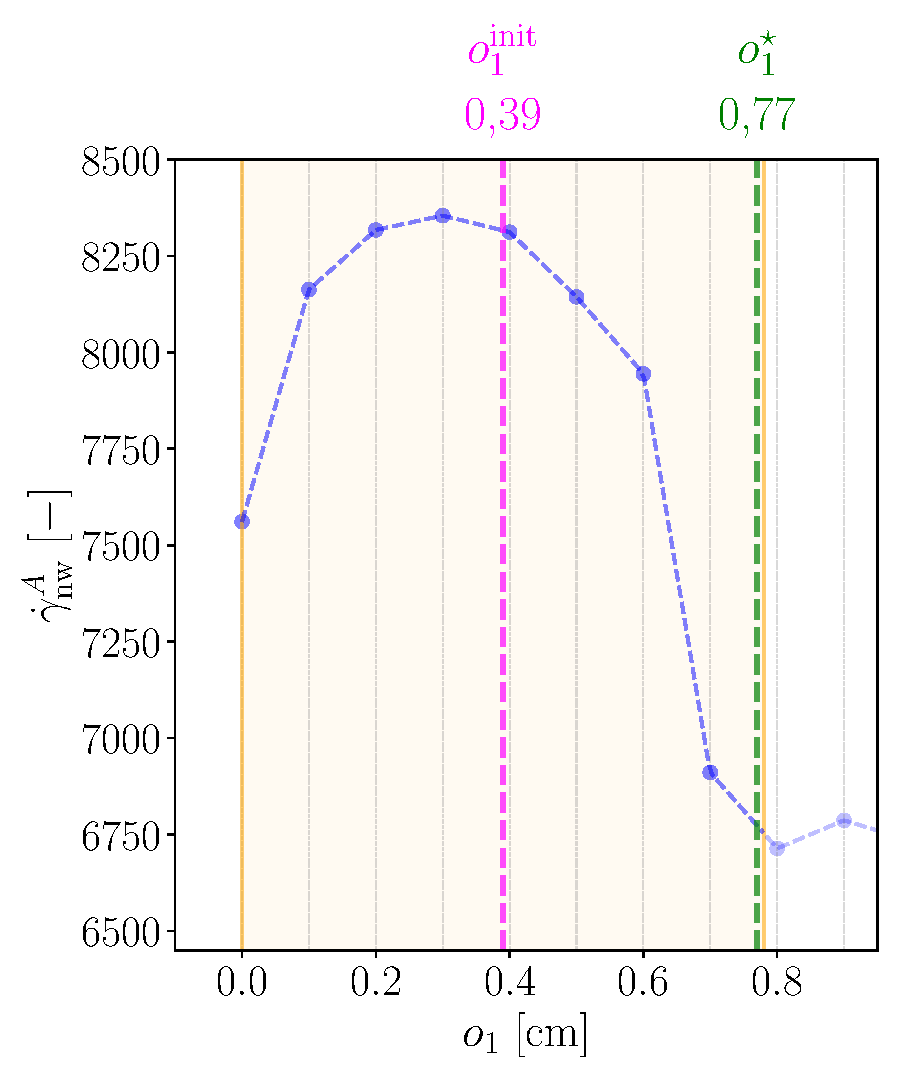
\includegraphics[
		width=\textwidth,
		trim={0mm 0mm 0mm -13mm}, clip
		]{figures/mean_stress_3_interpolated_point.pdf}
	\end{subfigure}\hfill%
	\begin{subfigure}{0.52\textwidth}
		\centering
		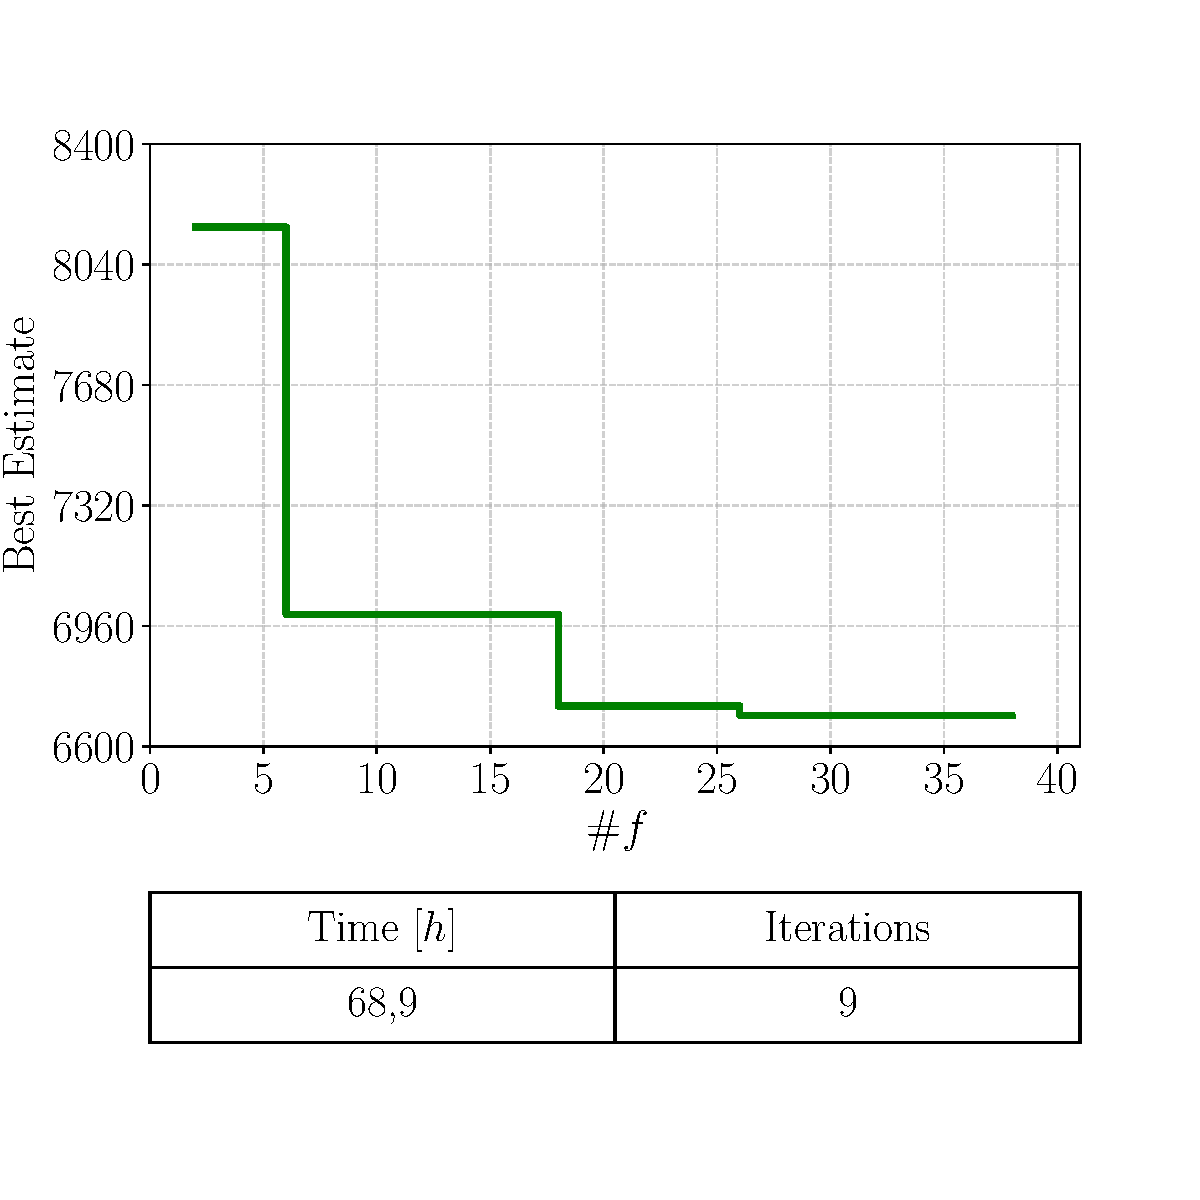
\includegraphics[
		width=1.05\textwidth,
		trim={0mm 25mm 0mm 0mm}, clip
		]{figures/optim_results/nm_sr.pdf}
	\end{subfigure}
	\vspace{2mm}
	\caption{Optimization results for Optimization Setup 1. The left plot compares the optimization result (marked point) with the previously sampled and interpolated objective function $\dot{\gamma}_{\text{max}}^{A}$ as a function of the parameter $o_1$. The right plot demonstrates the convergence of the optimization method, showing the best estimate against the number of objective function evaluations ($\# f$). The table summarizes the total elapsed time of the optimization algorithm (68,9 hours) and the number of iterations of the used method (9).}
\end{figure}
\newpage
\begin{optimproblem}{Basic cylindrical junction ($T^{A}_{\mathrm{turb}}$)}
	\vspace{2mm}
	Objective: Minimizing turbulent kinetic energy $T^{A}_{\mathrm{turb}}$.
	
	\vspace{2mm}
	Geometrical model:
	\begin{itemize}
		\item Model 1 as described in Section~\ref{mod:model1}.
		\item Optimization parameters: offset $o_1$.
	\end{itemize}
	Constraints:
	\begin{itemize}
		\item Offset constraint: $0{,}0~\text{cm} \leq o_1 \leq 2{,}4~\text{cm}$.
		\item Flow split constraint: $F^{\text{LPA}}_{\text{IVC}} \geq 25~\%$.
	\end{itemize}
	Optimization method:
	\begin{itemize}
		\item Nelder-Mead method as described in Section~\ref{framework} and Appendix~\ref{appendix C}.
	\end{itemize}
	Initial point: $o^{\text{init}}_{1}$ = 0{,}39 cm
	\label{optimprob:2}
\end{optimproblem}
\vspace{-5mm}

\begin{figure}[H]
	\centering
	\begin{subfigure}{0.46\textwidth}
		\centering
		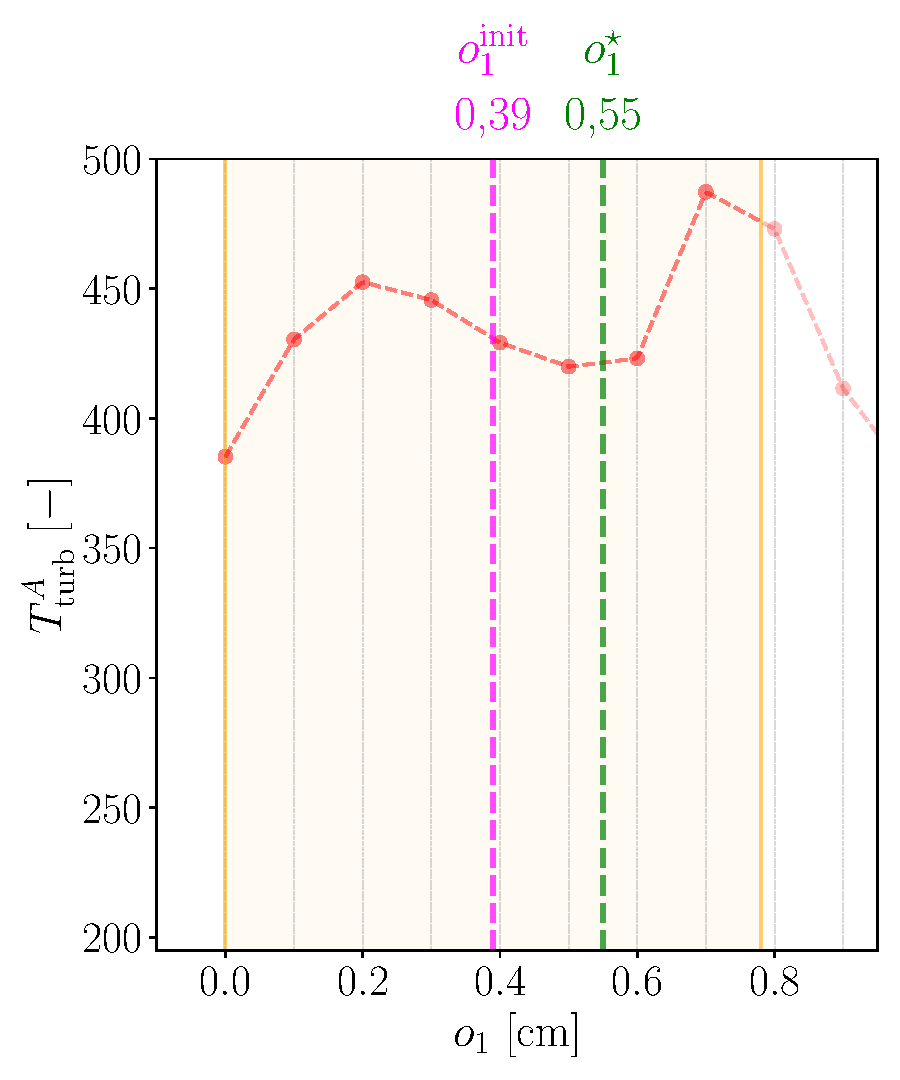
\includegraphics[
		width=\textwidth,
		trim={0mm 0mm 0mm -13mm}, clip
		]{figures/mean_turbulence_kinetic_energy_interpolated_point.pdf}
	\end{subfigure}\hfill%
	\begin{subfigure}{0.52\textwidth}
		\centering
		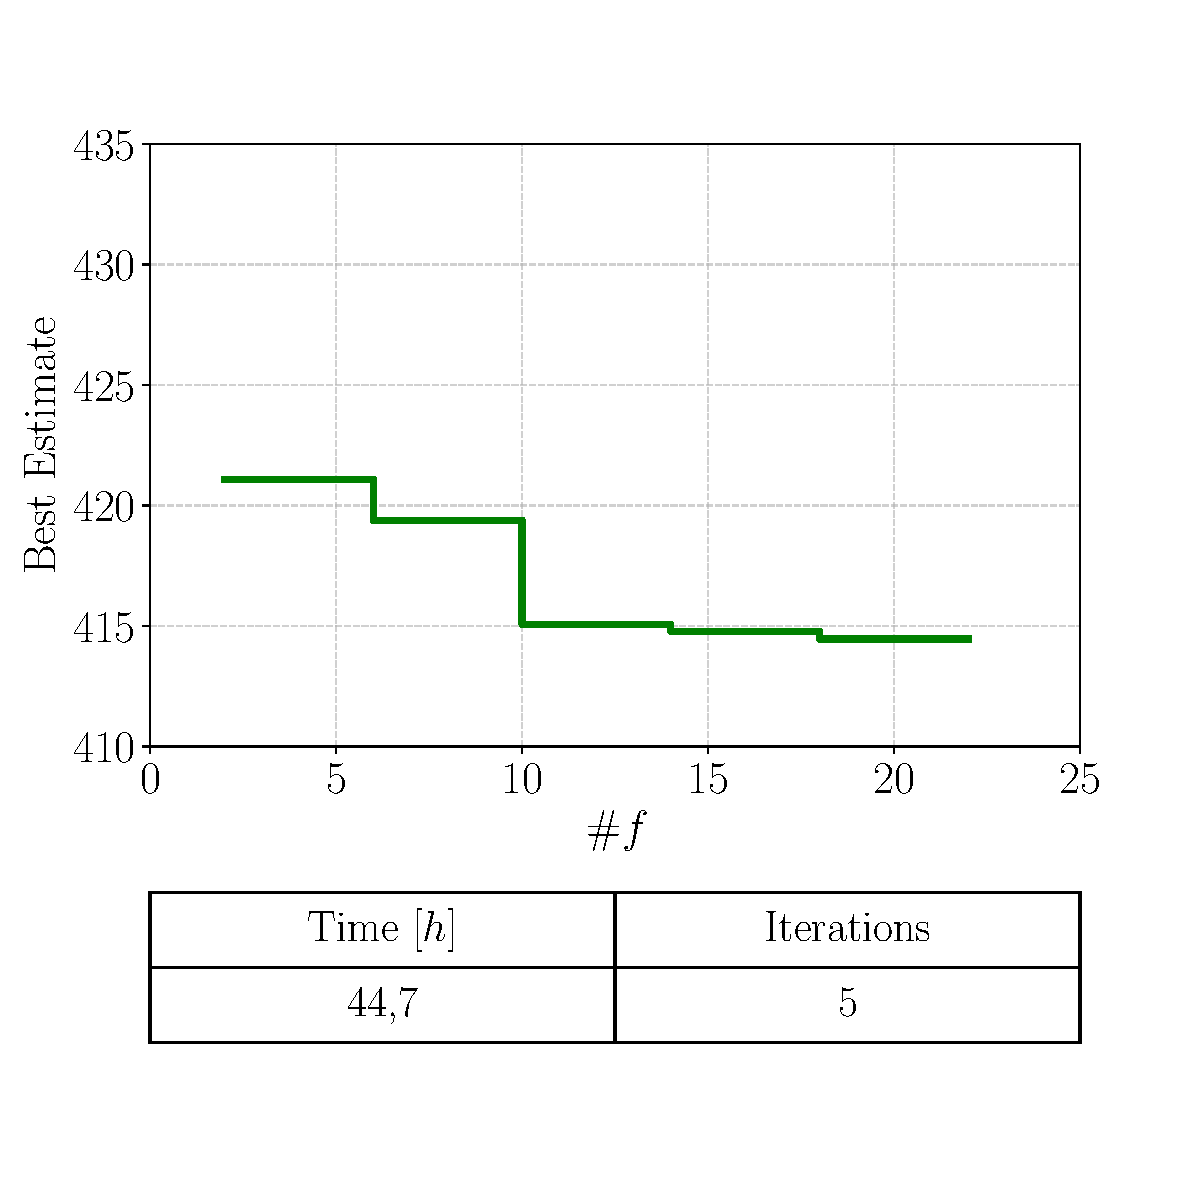
\includegraphics[
		width=1.05\textwidth,
		trim={0mm 25mm 0mm 0mm}, clip
		]{figures/optim_results/nm_tke.pdf}
	\end{subfigure}
	\vspace{2mm}
	\caption{Optimization results for Optimization Setup 2. The left plot compares the optimization result (marked point) with the previously sampled and interpolated objective function $\dot{\gamma}_{\text{max}}^{A}$ as a function of the parameter $o_1$. The right plot demonstrates the convergence of the optimization method, showing the best estimate against the number of objective function evaluations ($\# f$). The table summarizes the total elapsed time of the optimization algorithm (44,7 hours) and the number of iterations of the used method (5).}
\end{figure}
\newpage
\begin{optimproblem}{Basic cylindrical junction ($\dot{\gamma}^{A}_{\text{nw}}$)}
	\vspace{2mm}
	Objective: Minimizing turbulent kinetic energy $\dot{\gamma}^{A}_{\text{nw}}$.
	
	\vspace{2mm}
	Geometrical model:
	\begin{itemize}
		\item Model 1 as described in Section~\ref{mod:model1}.
		\item Optimization parameters: offset $o_1$.
	\end{itemize}
	Constraints:
	\begin{itemize}
		\item Offset constraint: $0{,}0~\text{cm} \leq o_1 \leq 2{,}4~\text{cm}$.
		\item Flow split constraint: $F^{\text{LPA}}_{\text{IVC}} \geq 25~\%$.
	\end{itemize}
	Optimization method:
	\begin{itemize}
		\item MADS method described in Section~\ref{framework}.
	\end{itemize}
	Initial point: $o^{\text{init}}_{1}$ = 0{,}39 cm
	\label{optimprob:3}
\end{optimproblem}

\begin{figure}[H]
	\centering
	\begin{subfigure}{0.47\textwidth}
		\centering
		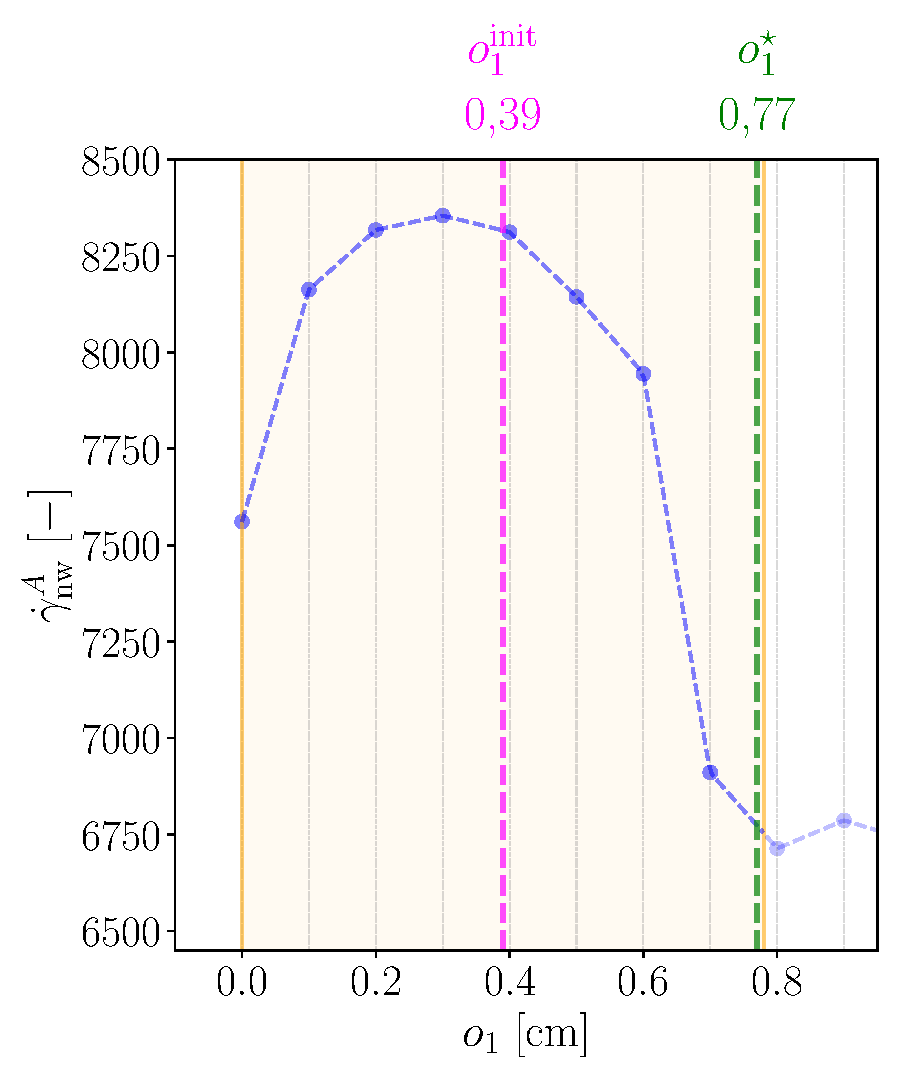
\includegraphics[
		width=\textwidth,
		trim={0mm 0mm 0mm -23mm}, clip
		]{figures/mean_stress_3_interpolated_point.pdf}
	\end{subfigure}\hfill%
	\begin{subfigure}{0.52\textwidth}
		\centering
		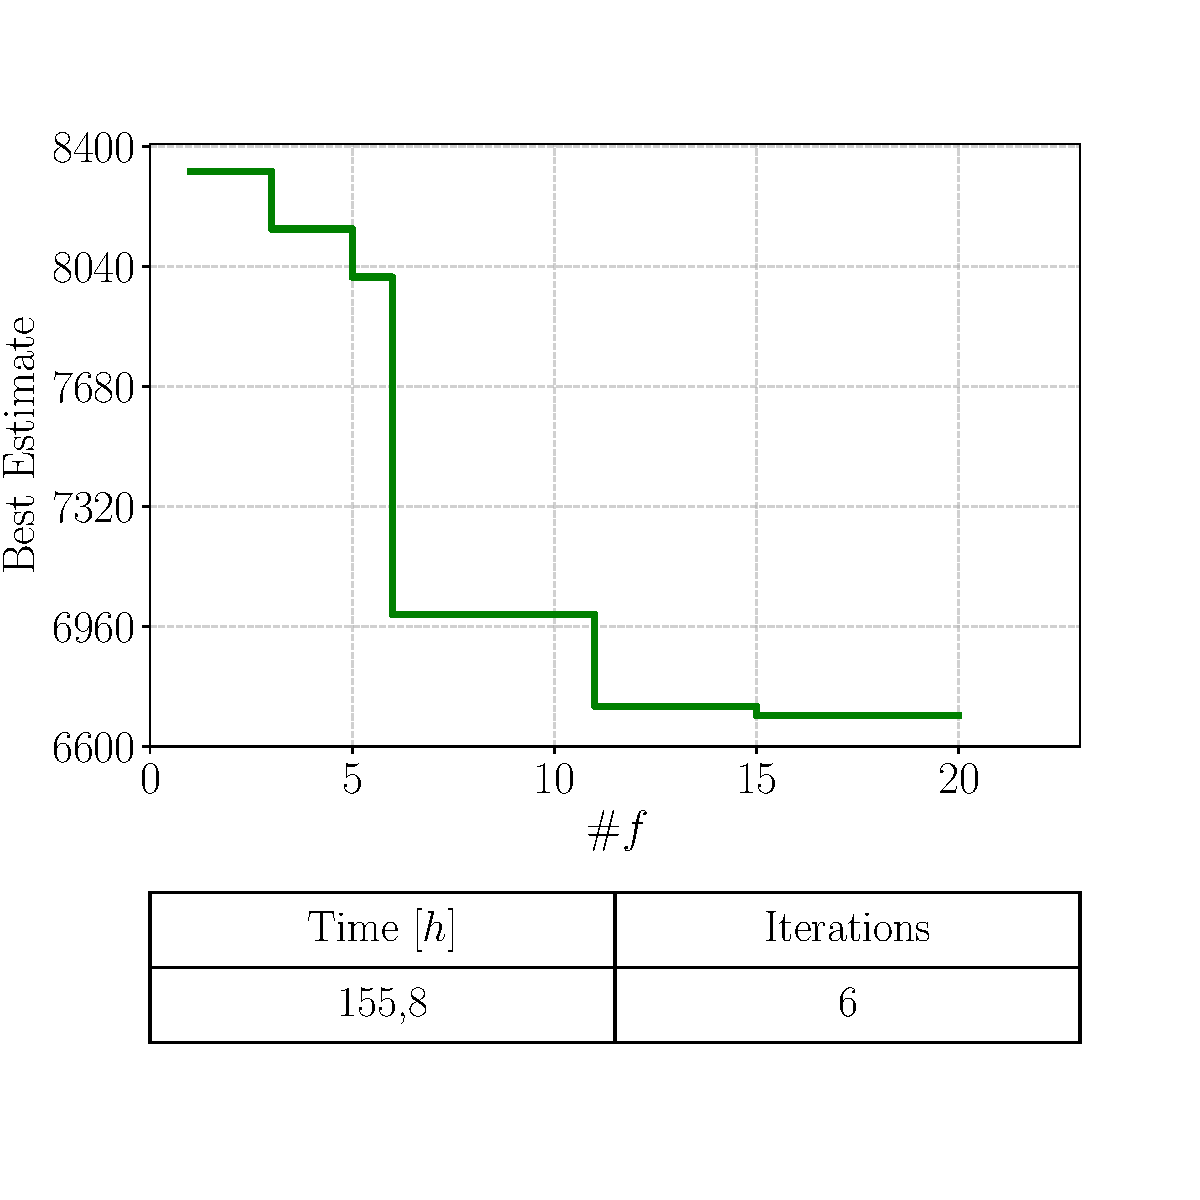
\includegraphics[
		width=1.05\textwidth,
		trim={0mm 25mm 0mm 0mm}, clip
		]{figures/optim_results/mads_sr.pdf}
	\end{subfigure}
	\vspace{2mm}
	\caption{Optimization results for Optimization Setup 3. The left plot compares the optimization result (marked point) with the previously sampled and interpolated objective function $\dot{\gamma}_{\text{max}}^{A}$ as a function of the parameter $o_1$. The right plot demonstrates the convergence of the optimization method, showing the best estimate against the number of objective function evaluations ($\# f$). The table summarizes the total elapsed time of the optimization algorithm (155,8 hours) and the number of iterations of the used method (6).}
\end{figure}
\newpage


\begin{optimproblem}{Basic cylindrical junction ($T^{A}_{\mathrm{turb}}$)}
	\vspace{2mm}
	Objective: Minimizing turbulent kinetic energy $T^{A}_{\mathrm{turb}}$.
	
	\vspace{2mm}
	Geometrical model:
	\begin{itemize}
		\item Model 1 as described in Section~\ref{mod:model1}.
		\item Optimization parameters: offset $o_1$.
	\end{itemize}
	Constraints:
	\begin{itemize}
		\item Offset constraint: $0{,}0~\text{cm} \leq o_1 \leq 2{,}4~\text{cm}$.
		\item Flow split constraint: $F^{\text{LPA}}_{\text{IVC}} \geq 25~\%$.
	\end{itemize}
	Optimization method:
	\begin{itemize}
		\item MADS method described in Section~\ref{framework}.
	\end{itemize}
	Initial point: $o^{\text{init}}_{1}$ = 0{,}39 cm
	\label{optimprob:4}
\end{optimproblem}
\vspace{-5mm}

\begin{figure}[H]
	\centering
	\begin{subfigure}{0.46\textwidth}
		\centering
		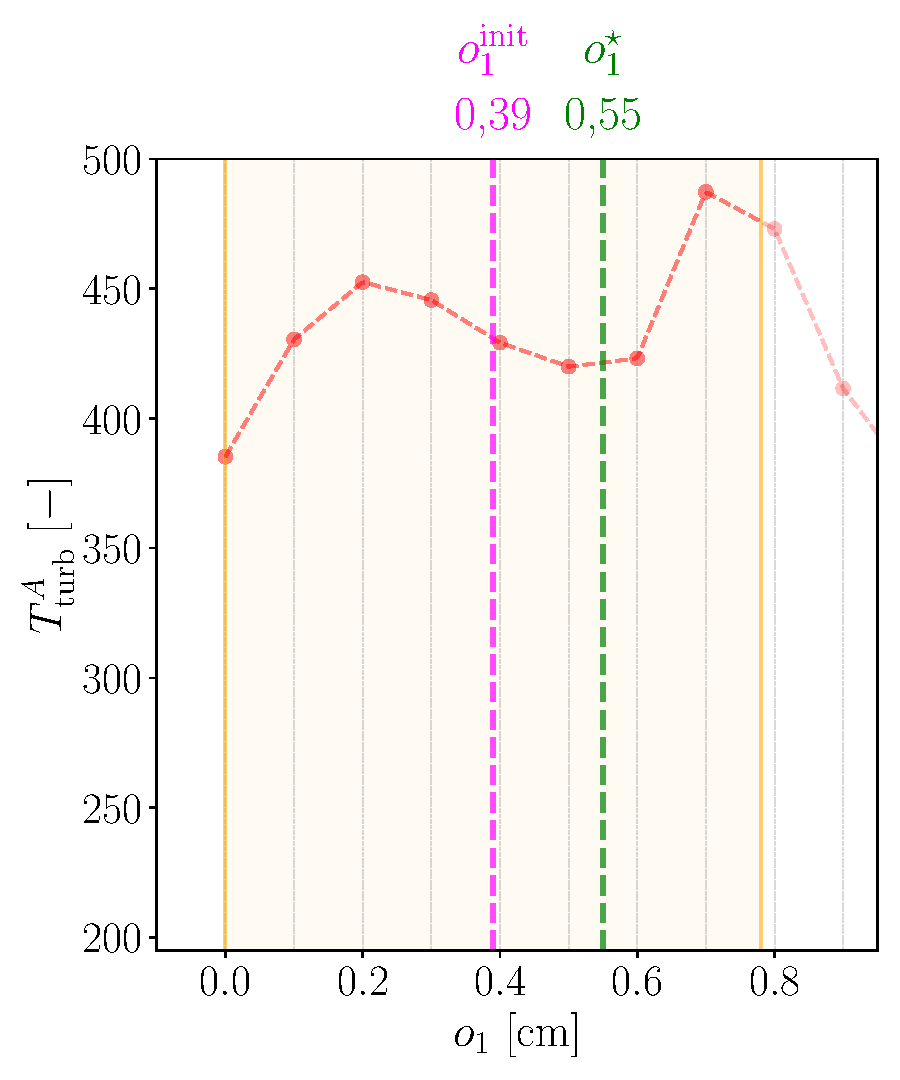
\includegraphics[
		width=\textwidth,
		trim={0mm 0mm 0mm -13mm}, clip
		]{figures/mean_turbulence_kinetic_energy_interpolated_point.pdf}
	\end{subfigure}\hfill%
	\begin{subfigure}{0.52\textwidth}
		\centering
		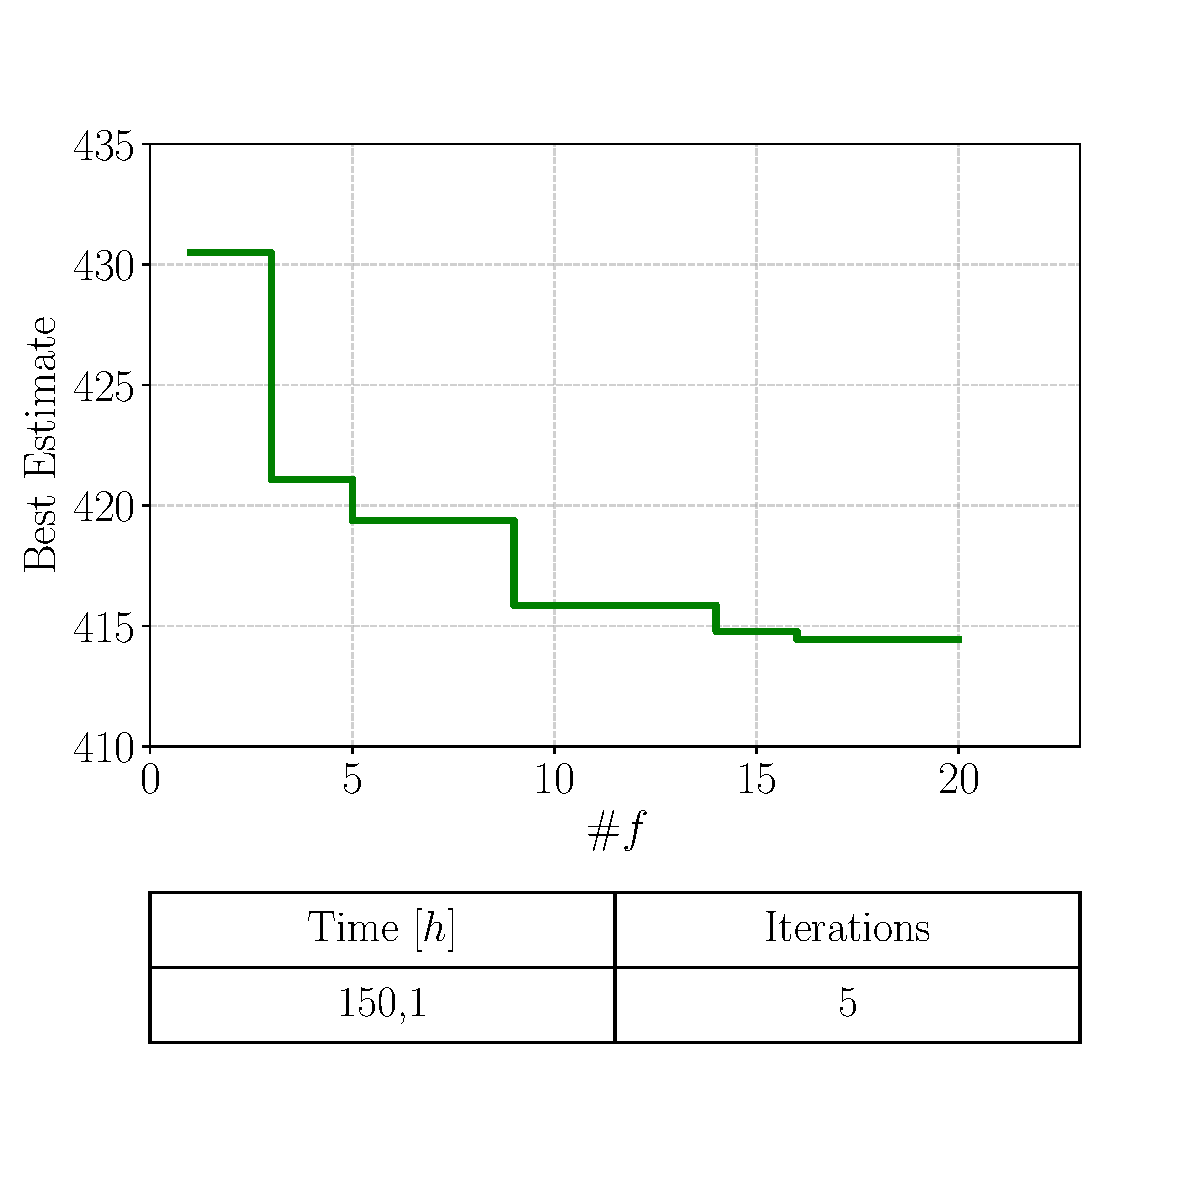
\includegraphics[
		width=1.05\textwidth,
		trim={0mm 25mm 0mm 0mm}, clip
		]{figures/optim_results/mads_tke.pdf}
	\end{subfigure}
	\vspace{2mm}
	\caption{Optimization results for Optimization Setup 4. The left plot compares the optimization result (marked point) with the previously sampled and interpolated objective function $\dot{\gamma}_{\text{max}}^{A}$ as a function of the parameter $o_1$. The right plot demonstrates the convergence of the optimization method, showing the best estimate against the number of objective function evaluations ($\# f$). The table summarizes the total elapsed time of the optimization algorithm (150,1 hours) and the number of iterations of the used method (5).}
\end{figure}
\newpage




From the optimization results, it can be observed that both the custom Nelder-Mead algorithm and the MADS method, when starting from the same initial point, resulted in the same outcomes for both the near-wall shear rate and turbulent kinetic energy minimization problems. However, for the turbulent kinetic energy objective, both methods converged to \(o_{1}^{\star} = 0{,}55\,\mathrm{cm}\), even though for the given constraints the true minimum is expected to be at \(o_{1}^{\star} = 0{,}0\,\mathrm{cm}\). This discrepancy is a direct consequence of the fact that neither Nelder-Mead nor MADS is a guaranteed global optimizer \cite{derivative-free-review}. In the case of the near-wall shear rate minimization, both methods identified the minimum at \(o_{1}^{\star} = 0{,}77\,\mathrm{cm}\), which aligns with expectations based on the interpolated sampled data.

It is worth noting that the MADS method consistently reached its predefined maximum number of objective function evaluations, leading to notably longer run times than the Nelder-Mead method. This difference stems from the fact that the current MADS method implementation runs sequentially. If MADS method were parallelized to allow simultaneous function evaluations, its overall execution time could be significantly reduced, potentially making it superior to the parallelized Nelder-Mead approach.